% =====================================================================
%  The Pitfalls of SHAP in Credit-Risk (PD) Models
%  Data Science Summit AI Edition  ·  online talk  ·  ~30 min
%
%  COMPILE:  xelatex shap_pitfalls.tex   (run twice for slide numbers)
% =====================================================================
\documentclass[aspectratio=169,11pt]{beamer}

\usepackage{fontspec}
\usepackage{tikz}
\usetikzlibrary{calc}
\usepackage[most]{tcolorbox}
\usepackage{pifont}
\usepackage{microtype}

% ---------------------------------------------------------------------
%  FONTS  (Carlito = clean, Calibri-metric; swap here if you prefer)
% ---------------------------------------------------------------------
\setsansfont{Carlito}[BoldFont=Carlito Bold, ItalicFont=Carlito Italic]
\setmonofont{DejaVu Sans Mono}[Scale=0.85]
\renewcommand{\familydefault}{\sfdefault}

% ---------------------------------------------------------------------
%  COLOR PALETTE  (one place to restyle the whole deck)
% ---------------------------------------------------------------------
\definecolor{nightbg}{HTML}{0E1525}% deep navy-black background
\definecolor{panel}{HTML}{18233F}  % card / panel fill
\definecolor{ink}{HTML}{EEF2FA}    % near-white body text
\definecolor{muted}{HTML}{8A97AD}  % slate captions / footers
\definecolor{gold}{HTML}{F5B500}   % primary brand accent
\definecolor{coral}{HTML}{FB5A54}  % danger
\definecolor{mint}{HTML}{2BD4B4}   % remedy / glass box
\definecolor{sky}{HTML}{5B8DEF}    % "what is SHAP" / neutral highlight

% ---------------------------------------------------------------------
%  BEAMER THEME  (dark throughout, no clutter)
% ---------------------------------------------------------------------
\setbeamercolor{background canvas}{bg=nightbg}
\setbeamercolor{normal text}{fg=ink}
\setbeamercolor{frametitle}{fg=ink}
\setbeamercolor{itemize item}{fg=gold}
\setbeamercolor{itemize subitem}{fg=muted}
\setbeamertemplate{navigation symbols}{}
\setbeamertemplate{itemize item}{\textcolor{gold}{\textbf{--}}}
\setbeamertemplate{itemize subitem}{\textcolor{muted}{\textbf{\textperiodcentered}}}
\setbeamerfont{frametitle}{series=\bfseries, size=\Large}
\setbeamerfont{itemize/enumerate body}{size=\large}

% frame title: bold, white, with breathing room (no accent rule lines)
\setbeamertemplate{frametitle}{%
  \vspace*{0.55cm}\hspace*{0.1cm}%
  \begin{minipage}{0.93\paperwidth}
    \raggedright\usebeamerfont{frametitle}\insertframetitle\par
  \end{minipage}\vspace*{0.15cm}}

% footer: talk tag (left) + slide number (right) in muted slate
\setbeamertemplate{footline}{%
  \hbox to \paperwidth{\hspace*{0.6cm}%
    \textcolor{muted}{\footnotesize The Scorecard Illusion}\hfill
    \textcolor{muted}{\footnotesize\insertframenumber}\hspace*{0.6cm}}%
  \vspace*{0.14cm}}

% ---------------------------------------------------------------------
%  HELPER MACROS
% ---------------------------------------------------------------------
% muted per-slide citation line, pinned near the bottom
\newcommand{\srcline}[1]{%
  \begin{textblock*}{14.8cm}(0.8cm,7.92cm)
    \textcolor{muted}{\scriptsize #1}
  \end{textblock*}}

% rule-to-remember callout (mint)
\newtcolorbox{rulebox}{
  enhanced, colback=panel, colframe=mint, boxrule=1pt, arc=4pt,
  left=10pt, right=10pt, top=7pt, bottom=7pt,
  coltext=ink, fontupper=\large}

% danger / warning callout (coral)
\newtcolorbox{warnbox}{
  enhanced, colback=panel, colframe=coral, boxrule=1pt, arc=4pt,
  left=10pt, right=10pt, top=7pt, bottom=7pt,
  coltext=ink, fontupper=\large}

% neutral fact callout (gold)
\newtcolorbox{factbox}{
  enhanced, colback=panel, colframe=gold, boxrule=1pt, arc=4pt,
  left=10pt, right=10pt, top=7pt, bottom=7pt,
  coltext=ink, fontupper=\large}

% big stat callout:  \stat{99.5\%}{zeros in training}
\newcommand{\stat}[2]{%
  \begin{minipage}[t]{0.26\textwidth}\centering
    {\fontsize{34}{38}\selectfont\bfseries\textcolor{gold}{#1}}\\[2pt]
    {\small\textcolor{muted}{#2}}
  \end{minipage}}

\usepackage[absolute,overlay]{textpos}
\setlength{\TPHorizModule}{1cm}\setlength{\TPVertModule}{1cm}

% ---------------------------------------------------------------------
%  REUSABLE VISUALS  (native TikZ — edit freely, no external images)
% ---------------------------------------------------------------------
% A "black box": feature dots flow in, a single score comes out.
\newcommand{\blackboxviz}{%
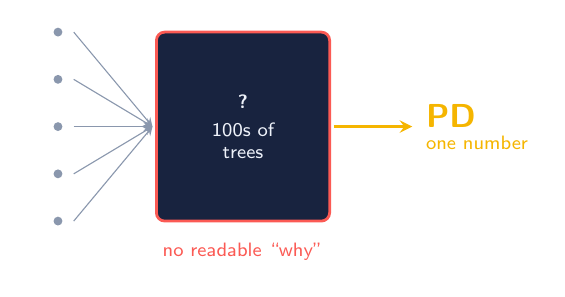
\begin{tikzpicture}[font=\scriptsize]
  \foreach \y in {0.4,1.0,1.6,2.2,2.8}{
    \fill[muted] (-0.15,\y) circle (1.6pt);
    \draw[muted,->,>=stealth] (0.05,\y) -- (1.05,1.6);}
  \node[text=muted, anchor=east] at (-0.25,1.6) {\,};
  \node[anchor=center, fill=panel, draw=coral, line width=1pt,
        rounded corners=3pt, minimum width=2.2cm, minimum height=2.4cm,
        text=ink, align=center] (bb) at (2.2,1.6)
        {\bfseries ?\\[2pt]\scriptsize 100s of\\\scriptsize trees};
  \draw[gold,->,>=stealth,line width=1pt] (3.35,1.6) -- (4.35,1.6);
  \node[text=gold, anchor=west, align=left] at (4.4,1.6)
        {\large\bfseries PD\\\scriptsize one number};
  \node[text=coral, anchor=north] at (2.2,0.25) {\scriptsize no readable ``why''};
\end{tikzpicture}}

% Connected SHAP waterfall (base -> +/- contributions -> f(x))
\newcommand{\waterfallviz}{%
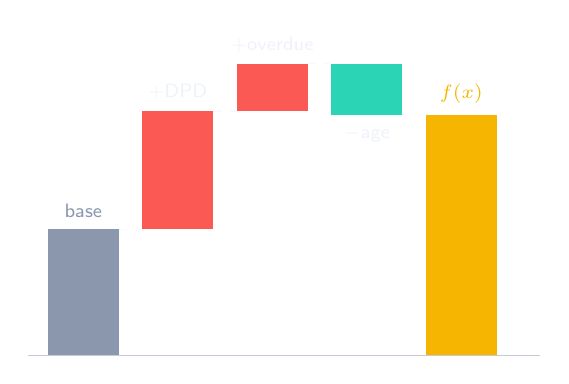
\begin{tikzpicture}[font=\scriptsize]
  \draw[muted,opacity=0.5] (-0.1,0) -- (6.4,0);
  % helper: each step drawn as a bar from prev level to new level
  % base
  \fill[muted] (0.15,0) rectangle (1.05,1.6);
  \node[text=muted,anchor=south] at (0.6,1.62){base};
  % +max DPD (up, coral)
  \fill[coral] (1.35,1.6) rectangle (2.25,3.1);
  \draw[ink,dashed,opacity=0.4] (1.05,1.6)--(1.35,1.6);
  \node[text=ink,anchor=south] at (1.8,3.12){\scriptsize +DPD};
  % +overdue (up, coral)
  \fill[coral] (2.55,3.1) rectangle (3.45,3.7);
  \draw[ink,dashed,opacity=0.4] (2.25,3.1)--(2.55,3.1);
  \node[text=ink,anchor=south] at (3.0,3.72){\scriptsize +overdue};
  % -age (down, mint)
  \fill[mint] (3.75,3.7) rectangle (4.65,3.05);
  \draw[ink,dashed,opacity=0.4] (3.45,3.7)--(3.75,3.7);
  \node[text=ink,anchor=north] at (4.2,3.03){\scriptsize $-$age};
  \draw[ink,dashed,opacity=0.4] (4.65,3.05)--(4.95,3.05);
  % f(x) total (gold)
  \fill[gold] (4.95,0) rectangle (5.85,3.05);
  \node[text=gold,anchor=south] at (5.4,3.07){\scriptsize $f(x)$};
\end{tikzpicture}}

% Two-panel: assumed linear effect vs the model's real, kinked effect
\newcommand{\whatifviz}{%
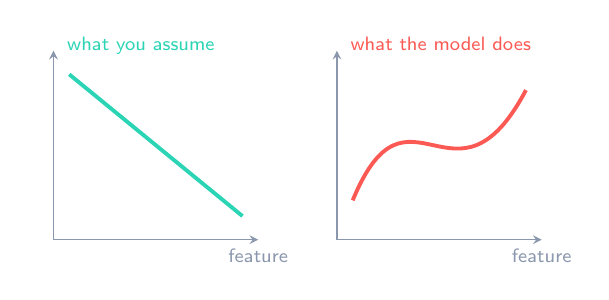
\begin{tikzpicture}[font=\scriptsize]
  % left panel: assumed
  \draw[muted,->,>=stealth] (0,0) -- (2.6,0) node[anchor=north,text=muted]{feature};
  \draw[muted,->,>=stealth] (0,0) -- (0,2.4) node[anchor=east,text=muted,rotate=90,yshift=6pt]{};
  \draw[mint,line width=1.4pt] (0.2,2.1) -- (2.4,0.3);
  \node[text=mint,anchor=north west] at (0.05,2.7){\scriptsize what you assume};
  % right panel: reality
  \begin{scope}[xshift=3.6cm]
   \draw[muted,->,>=stealth] (0,0) -- (2.6,0) node[anchor=north,text=muted]{feature};
   \draw[muted,->,>=stealth] (0,0) -- (0,2.4);
   \draw[coral,line width=1.4pt] (0.2,0.5) .. controls (0.9,2.2) and (1.5,0.2) .. (2.4,1.9);
   \node[text=coral,anchor=north west] at (0.05,2.7){\scriptsize what the model does};
  \end{scope}
\end{tikzpicture}}

% Two SHAP bar-sets (Mon vs Tue): one input changed, many bars move
\newcommand{\daydayviz}{%
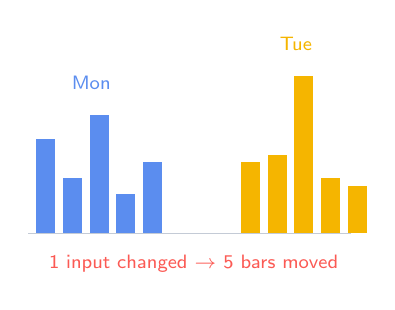
\begin{tikzpicture}[font=\scriptsize]
  % Monday
  \foreach \i/\h in {0/1.2,1/0.7,2/1.5,3/0.5,4/0.9}{
     \fill[sky] ({\i*0.34},0) rectangle ({\i*0.34+0.24},\h);}
  \node[text=sky,anchor=south] at (0.7,1.7){Mon};
  % Tuesday (only feature 2 truly changed, yet all shift)
  \begin{scope}[xshift=2.6cm]
   \foreach \i/\h in {0/0.9,1/1.0,2/2.0,3/0.7,4/0.6}{
     \fill[gold] ({\i*0.34},0) rectangle ({\i*0.34+0.24},\h);}
   \node[text=gold,anchor=south] at (0.7,2.2){Tue};
  \end{scope}
  \draw[muted,opacity=0.5] (-0.1,0) -- (4.0,0);
  \node[text=coral,anchor=north,align=center] at (2.0,-0.15)
       {\scriptsize 1 input changed $\to$ 5 bars moved};
\end{tikzpicture}}

% Horizontal importance ranking: lonely "age" tops a split DPD family
% #1 = title colour key not needed; draws fixed illustrative bars
\newcommand{\impranking}{%
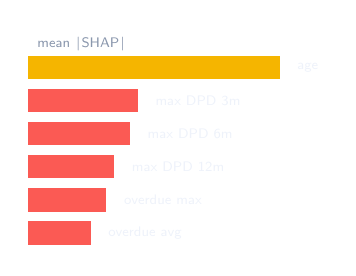
\begin{tikzpicture}[font=\scriptsize]
  % bars: name / width / colour
  \foreach \i/\name/\w/\c in {
     0/{age}/3.2/gold,
     1/{max DPD 3m}/1.4/coral,
     2/{max DPD 6m}/1.3/coral,
     3/{max DPD 12m}/1.1/coral,
     4/{overdue max}/1.0/coral,
     5/{overdue avg}/0.8/coral}{
       \pgfmathsetmacro\yy{2.5-\i*0.42}
       \fill[\c] (0,\yy) rectangle (\w,\yy+0.3);
       \node[text=ink,anchor=west,font=\tiny] at (\w+0.1,\yy+0.15){\name};
  }
  \node[text=muted,anchor=west,font=\tiny] at (0,2.95){mean $|$SHAP$|$};
\end{tikzpicture}}

% Two mini histograms: training (spike at 0) vs production (spread)
\newcommand{\histshift}{%
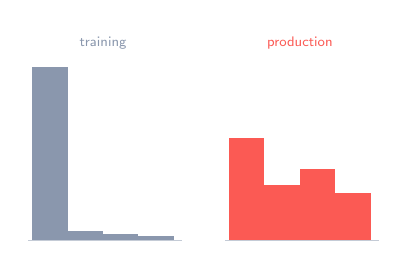
\begin{tikzpicture}[font=\scriptsize]
  % training
  \fill[muted] (0,0) rectangle (0.45,2.2);
  \foreach \i/\h in {1/0.12,2/0.08,3/0.05}{\fill[muted] ({\i*0.45},0) rectangle ({\i*0.45+0.45},\h);}
  \draw[muted,opacity=0.5] (-0.05,0)--(1.9,0);
  \node[text=muted,anchor=south,font=\tiny] at (0.9,2.3){training};
  % production
  \begin{scope}[xshift=2.5cm]
   \fill[coral] (0,0) rectangle (0.45,1.3);
   \foreach \i/\h in {1/0.7,2/0.9,3/0.6}{\fill[coral] ({\i*0.45},0) rectangle ({\i*0.45+0.45},\h);}
   \draw[muted,opacity=0.5] (-0.05,0)--(1.9,0);
   \node[text=coral,anchor=south,font=\tiny] at (0.9,2.3){production};
  \end{scope}
\end{tikzpicture}}

% Dependence scatter where the SHAP trend flips sign by an interacting group
\newcommand{\signflipviz}{%
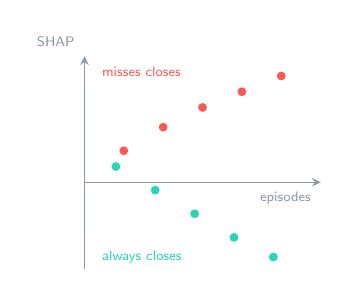
\begin{tikzpicture}[font=\scriptsize]
  \draw[muted,->,>=stealth] (0,0) -- (3.0,0) node[anchor=north east,text=muted,font=\tiny]{episodes};
  \draw[muted,->,>=stealth] (0,-1.1) -- (0,1.6) node[anchor=south east,text=muted,font=\tiny]{SHAP};
  \draw[muted,opacity=0.4] (0,0)--(3.0,0);
  % group A: "always closed on time" -> negative trend (mint)
  \foreach \x/\y in {0.4/0.2,0.9/-0.1,1.4/-0.4,1.9/-0.7,2.4/-0.95}{\fill[mint] (\x,\y) circle (1.6pt);}
  % group B: "missed closes" -> positive trend (coral)
  \foreach \x/\y in {0.5/0.4,1.0/0.7,1.5/0.95,2.0/1.15,2.5/1.35}{\fill[coral] (\x,\y) circle (1.6pt);}
  \node[text=mint,anchor=west,font=\tiny] at (0.1,-0.95){always closes};
  \node[text=coral,anchor=west,font=\tiny] at (0.1,1.4){misses closes};
\end{tikzpicture}}

% EBM-style per-feature shape function (a drawn, exact curve)
\newcommand{\shapefn}{%
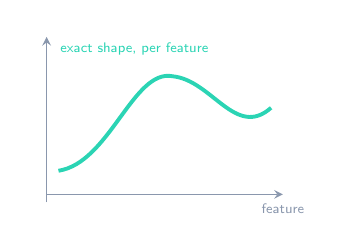
\begin{tikzpicture}[font=\scriptsize]
  \draw[muted,->,>=stealth] (0,0) -- (3.0,0) node[anchor=north,text=muted,font=\tiny]{feature};
  \draw[muted,->,>=stealth] (0,-0.1) -- (0,2.0) node[anchor=east,text=muted,font=\tiny]{};
  \draw[mint,line width=1.4pt]
     (0.15,0.3) .. controls (0.8,0.4) and (1.1,1.6) .. (1.6,1.5)
                .. controls (2.1,1.45) and (2.4,0.7) .. (2.85,1.1);
  \node[text=mint,anchor=north west,font=\tiny] at (0.05,2.05){exact shape, per feature};
\end{tikzpicture}}

% "One question it answers, many it doesn't" hub (for the silver-bullet slide)
\newcommand{\hubviz}{%
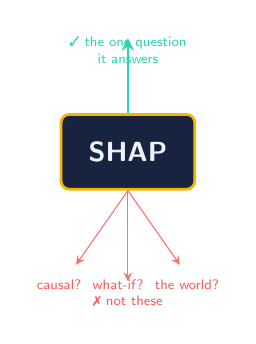
\begin{tikzpicture}[font=\scriptsize]
  \node[fill=panel, draw=gold, line width=1pt, rounded corners=3pt,
        minimum width=1.7cm, minimum height=0.95cm, text=ink, font=\bfseries]
        (s) at (0,0) {SHAP};
  % the one good question (mint, up)
  \draw[mint,->,>=stealth,line width=1pt] (s.north) -- ++(0,0.95);
  \node[text=mint,anchor=south,align=center,font=\tiny] at (0,1.0)
        {\textbf{\ding{51}} the one question\\ it answers};
  % the questions it does NOT answer (coral fan, down)
  \foreach \a in {-125,-90,-55}{
     \draw[coral,opacity=0.85,->,>=stealth] (s.south) -- ++(\a:1.15cm);}
  \node[text=coral,anchor=north,align=center,font=\tiny] at (0,-1.5)
        {causal? \ what-if? \ the world?\\ \textbf{\ding{55}} not these};
\end{tikzpicture}}

% Population SHAP distribution drifting month-over-month (explanation shift)
\newcommand{\driftviz}{%
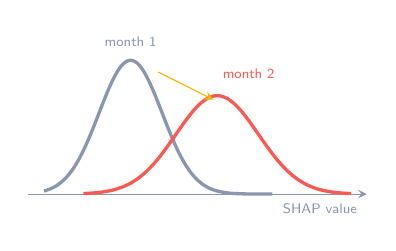
\begin{tikzpicture}[font=\scriptsize]
  \draw[muted,->,>=stealth] (-0.1,0) -- (4.2,0)
        node[anchor=north east,text=muted,font=\tiny]{SHAP value};
  % month 1 (muted bell, left)
  \draw[muted,line width=1.2pt] plot[smooth,domain=0.1:3.0,samples=40]
        (\x, {1.7*exp(-((\x-1.2)^2)/0.32)});
  \node[text=muted,anchor=south,font=\tiny] at (1.2,1.75){month 1};
  % month 2 (coral bell, shifted right + flatter = drift)
  \draw[coral,line width=1.2pt] plot[smooth,domain=0.6:4.0,samples=40]
        (\x, {1.25*exp(-((\x-2.3)^2)/0.55)});
  \node[text=coral,anchor=south,font=\tiny] at (2.7,1.35){month 2};
  \draw[gold,->,>=stealth] (1.55,1.55) -- (2.25,1.2);
\end{tikzpicture}}

% Big "no LLMs" prohibition sign
\newcommand{\noLLM}{%

\begin{tikzpicture}
  \node[text=ink] at (0,0) {\fontsize{58}{58}\selectfont\bfseries LLM};
  \draw[coral, line width=6pt] (0,0) circle (2.35cm);
  \draw[coral, line width=6pt] (135:2.35cm) -- (-45:2.35cm);
\end{tikzpicture}}

% Slide 15: many SHAPs moved, only one input moved -> watch inputs too
\newcommand{\watchinputs}{%
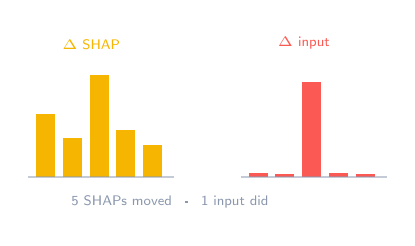
\begin{tikzpicture}[font=\scriptsize]
  \foreach \i/\h in {0/0.8,1/0.5,2/1.3,3/0.6,4/0.4}{
     \fill[gold] ({\i*0.34},0) rectangle ({\i*0.34+0.24},\h);}
  \node[text=gold,anchor=south,font=\tiny] at (0.7,1.5){$\Delta$ SHAP};
  \draw[muted,opacity=0.5] (-0.1,0)--(1.75,0);
  \begin{scope}[xshift=2.7cm]
   \foreach \i/\h in {0/0.05,1/0.04,2/1.2,3/0.05,4/0.04}{
      \fill[coral] ({\i*0.34},0) rectangle ({\i*0.34+0.24},\h);}
   \node[text=coral,anchor=south,font=\tiny] at (0.7,1.5){$\Delta$ input};
   \draw[muted,opacity=0.5] (-0.1,0)--(1.75,0);
  \end{scope}
  \node[text=muted,anchor=north,align=center,font=\tiny] at (1.7,-0.12)
       {5 SHAPs moved \, · \, 1 input did};
\end{tikzpicture}}

% Slide 22: a feature alone (= intuition) vs the same feature inside the full model
\newcommand{\alonevsmodel}{%
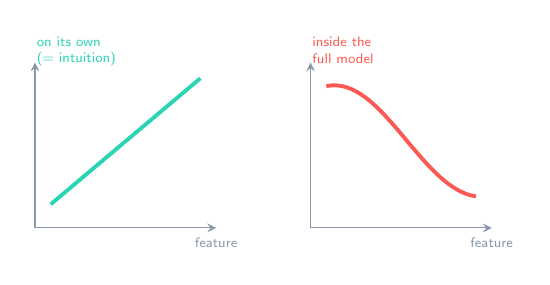
\begin{tikzpicture}[font=\scriptsize]
  \draw[muted,->,>=stealth] (0,0)--(2.3,0) node[anchor=north,text=muted,font=\tiny]{feature};
  \draw[muted,->,>=stealth] (0,0)--(0,2.1);
  \draw[mint,line width=1.4pt] (0.2,0.3)--(2.1,1.9);
  \node[text=mint,anchor=north west,font=\tiny,align=left] at (-0.1,2.55)
       {on its own\\(= intuition)};
  \begin{scope}[xshift=3.5cm]
   \draw[muted,->,>=stealth] (0,0)--(2.3,0) node[anchor=north,text=muted,font=\tiny]{feature};
   \draw[muted,->,>=stealth] (0,0)--(0,2.1);
   \draw[coral,line width=1.4pt] (0.2,1.8) .. controls (0.9,1.95) and (1.4,0.5) .. (2.1,0.4);
   \node[text=coral,anchor=north west,font=\tiny,align=left] at (-0.1,2.55)
        {inside the\\full model};
  \end{scope}
\end{tikzpicture}}

% Slide 18: importance ranking before vs after grouping correlated features
\newcommand{\groupedimp}{%
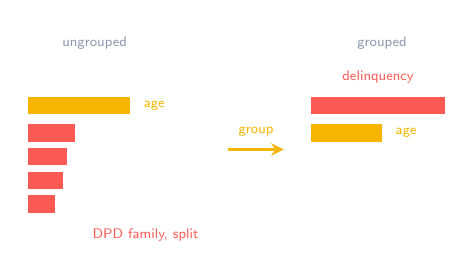
\begin{tikzpicture}[font=\tiny]
  % ----- ungrouped -----
  \node[text=muted,anchor=south] at (0.85,2.05){ungrouped};
  \fill[gold] (0,1.35) rectangle (1.3,1.57);
  \node[text=gold,anchor=west] at (1.35,1.46){age};
  \foreach \i/\w in {0/0.6,1/0.5,2/0.45,3/0.35}{
     \pgfmathsetmacro\yy{1.0-\i*0.30}
     \fill[coral] (0,\yy) rectangle (\w,\yy+0.22);}
  \node[text=coral,anchor=west] at (0.7,-0.18){DPD family, split}; 
  % arrow
  \draw[gold,->,>=stealth,line width=1pt] (2.55,0.9) -- (3.25,0.9);
  \node[text=gold,anchor=south,font=\tiny] at (2.9,0.95){group};
  % ----- grouped -----
  \begin{scope}[xshift=3.6cm]
   \node[text=muted,anchor=south] at (0.9,2.05){grouped};
   \node[text=coral,anchor=south,font=\tiny] at (0.85,1.62){delinquency};
   \fill[coral] (0,1.35) rectangle (1.7,1.57);
   \fill[gold] (0,1.0) rectangle (0.9,1.22);
   \node[text=gold,anchor=west] at (0.95,1.11){age};
  \end{scope}
\end{tikzpicture}}

% Slide: correlation makes SHAP sample feature combinations that never occur
\newcommand{\unrealviz}{%
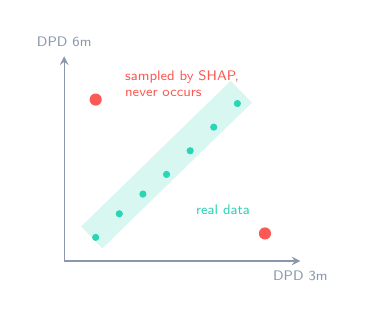
\begin{tikzpicture}[font=\tiny]
  \draw[muted,->,>=stealth] (0,0)--(3.0,0) node[anchor=north,text=muted,font=\tiny]{DPD 3m};
  \draw[muted,->,>=stealth] (0,0)--(0,2.6) node[anchor=south,text=muted,font=\tiny]{DPD 6m};
  % realistic, correlated cloud along the diagonal
  \draw[mint,opacity=0.18,line width=11pt] (0.35,0.3) -- (2.25,2.15);
  \foreach \x/\y in {0.4/0.3,0.7/0.6,1.0/0.85,1.3/1.1,1.6/1.4,1.9/1.7,2.2/2.0}{
     \fill[mint] (\x,\y) circle (1.3pt);}
  \node[text=mint,anchor=west,font=\tiny] at (1.55,0.65){real data};
  % unrealistic sampled points off the diagonal
  \foreach \x/\y in {2.55/0.35,0.4/2.05}{\fill[coral] (\x,\y) circle (2.2pt);}
  \node[text=coral,anchor=west,font=\tiny,align=left] at (0.65,2.25)
       {sampled by SHAP,\\ never occurs};
\end{tikzpicture}}

% full-bleed dark divider for each pitfall
% \dangerframe{number}{HEADLINE}{subtitle line}
\newcommand{\dangerframe}[3]{%
\begin{frame}[plain]
\begin{tikzpicture}[remember picture,overlay]
  \fill[nightbg] (current page.south west) rectangle (current page.north east);
  % faint oversized numeral motif
  \node[anchor=east, text=panel, scale=1] at ($(current page.east)+(-0.2,1.4)$)
       {\fontsize{300}{300}\selectfont\bfseries #1};
  \node[anchor=west, text=coral] at ($(current page.west)+(1.1,2.6)$)
       {\fontsize{26}{26}\selectfont\bfseries PITFALL\ \ \##1};
  \node[anchor=north west, text=ink, align=left] at ($(current page.west)+(1.0,1.95)$)
       {\fontsize{30}{36}\selectfont\bfseries\begin{minipage}{10.2cm}\raggedright #2\end{minipage}};
  \node[anchor=west, text=muted, align=left] at ($(current page.west)+(1.1,-2.7)$)
       {\large\begin{minipage}{10cm}\raggedright #3\end{minipage}};
\end{tikzpicture}
\end{frame}}

\title{The Scorecard Illusion}
\author{Daniel Wlaz\l o}

% =====================================================================
\begin{document}

% ---------- 1. TITLE -------------------------------------------------
\begin{frame}[plain]
\begin{tikzpicture}[remember picture,overlay]
  \fill[nightbg] (current page.south west) rectangle (current page.north east);
  % motif: a faint waterfall of bars behind the title
  \foreach \x/\h/\c in {6.8/1.2/coral, 7.7/2.1/coral, 8.6/1.0/mint, 9.5/2.6/mint, 10.4/1.6/gold}{
     \fill[\c, opacity=0.16] ($(current page.south west)+(\x,1.0)$) rectangle ++(0.55,\h);}
  \node[anchor=west, text=gold] at ($(current page.west)+(1.1,2.85)$)
       {\fontsize{14}{14}\selectfont\bfseries DATA SCIENCE SUMMIT · AI EDITION · ONLINE};
  \node[anchor=west, text=ink, align=left] at ($(current page.west)+(1.05,1.05)$)
       {\fontsize{37}{41}\selectfont\bfseries\begin{minipage}{12.8cm}\raggedright
        The Scorecard Illusion\end{minipage}};
  \node[anchor=west, text=gold, align=left] at ($(current page.west)+(1.1,-1.25)$)
       {\fontsize{19}{24}\selectfont\begin{minipage}{12.8cm}\raggedright
        Why SHAP values are not points --- and how they can fool you\end{minipage}};
  \node[anchor=west, text=muted, align=left] at ($(current page.west)+(1.12,-3.1)$)
       {\large Daniel Wlaz\l o\, ·\, Manager Data Science, Allegro Pay\\[2pt]
        \normalsize\itshape PhD candidate, SGH Warsaw School of Economics};
\end{tikzpicture}
\end{frame}

% ---------- 2. OPENING / HOOK ---------------------------------------
\begin{frame}[c]{}
\centering
\noLLM\\[18pt]
{\Large\textcolor{ink}{This talk is about \textbf{classic, tabular ML} --- not LLMs.}}\\[4pt]
{\large\textcolor{muted}{The ``boring'' models that still decide what happens to your money.}}
\note{[00:00--01:30] The confession: almost every talk here is about LLMs --- agents,
RAG, prompting. I came to talk about plain tabular gradient boosting, one row per
customer. And this ``boring'' ML still decides what happens to your money. Today:
SHAP --- a tool you all love --- and how it can fool you. Light, smile, move on.}
\end{frame}

% ---------- 3. THE PD MODEL / BLACK BOX -----------------------------
\begin{frame}{The setup: a PD model}
\large
\textbf{Probability of default} --- will this customer stop repaying within the next
12 months? It's fed by the customer's behavioural and credit history: delinquency
record, max DPD, overdue amounts, utilization, age.\\[14pt]
\begin{columns}[c]
\column{0.46\textwidth}
  \textcolor{muted}{\bfseries Logistic scorecard}\\
  \normalsize Readable, regulator-friendly --- \textcolor{coral}{but loses on
  performance.}\\[12pt]
  \textcolor{mint}{\bfseries XGBoost / LightGBM}\\
  \normalsize Higher Gini, catches hidden risk --- \textcolor{coral}{but it's a
  black box.}
\column{0.5\textwidth}
  \centering\blackboxviz
\end{columns}
\note{[01:30--04:30] Establish vocabulary. Gradient boosting wins on money; the cost is opacity.}
\end{frame}

% ---------- 4. WHY EXPLANATIONS ------------------------------------
\begin{frame}{Why we even need to explain it}
\large
Hundreds of trees voting. Nobody reads that off the cuff. Yet we \emph{must}
say why a customer was declined --- for three audiences:\\[14pt]
\begin{columns}[T]
\column{0.31\textwidth}
  {\bfseries\textcolor{gold}{Regulator}}\\[3pt]
  Prove the model isn't doing something stupid or discriminatory.
\column{0.31\textwidth}
  {\bfseries\textcolor{gold}{Business}}\\[3pt]
  Why did the model suddenly mass-reject this segment?
\column{0.31\textwidth}
  {\bfseries\textcolor{gold}{Customer}}\\[3pt]
  A \emph{specific} reason for a decline --- increasingly a legal right, not a courtesy.
\end{columns}
\vspace{14pt}
\hfill\textcolor{ink}{\large A black box you are obliged to explain. \textbf{Enter SHAP.}}
\srcline{EU AI Act 2024/1689 (Annex III 5b: credit scoring high-risk; Art.\ 86) · PL ustawa o kredycie konsumenckim, art.\ 9--10.}
\note{[Regulatory framing. AI Act Art. 86 applies from Aug 2027; PL art. 10 ust. 2 odsyła do art. 70a Prawa bankowego --- wyjaśnienie oceny zdolności kredytowej. Direction of thinking, not legal advice.]}
\end{frame}

% ---------- 5. WHAT IS SHAP ----------------------------------------
\begin{frame}{What SHAP is, in one breath}
\large
From \textbf{cooperative game theory}: split a payout among players, fairly, in
proportion to contribution.\\[10pt]
\begin{columns}[T]
\column{0.5\textwidth}
  \textcolor{sky}{\bfseries The rules it obeys}
  \begin{itemize}
    \item No contribution $\Rightarrow$ zero
    \item Equal contribution $\Rightarrow$ equal share
    \item Shares sum to the whole payout
  \end{itemize}
\column{0.5\textwidth}
  \textcolor{sky}{\bfseries Mapped to our model}
  \begin{itemize}
    \item Game $=$ the prediction
    \item Players $=$ the features
    \item Payout $=$ prediction $-$ average
  \end{itemize}
\end{columns}
\vspace{10pt}
\begin{factbox}
Additivity: base value $+$ contributions $=$ \emph{exactly} this customer's prediction.
\end{factbox}
\note{[04:30--08:00] Keep game theory to intuition. Do NOT derive the sum-over-subsets formula.}
\end{frame}

% ---------- 6. WATERFALL + WHY GREAT --------------------------------
\begin{frame}{One customer, decomposed --- and why it's great}
\begin{columns}[c]
\column{0.54\textwidth}
\centering\waterfallviz
\column{0.44\textwidth}
\large
Local explanations. Global summaries when averaged. Fast for trees.\\[10pt]
\textcolor{mint}{\bfseries If I had to pick one explainer for tabular ML, I'd pick SHAP.}\\[10pt]
\textcolor{muted}{So why throw mud at it for 20 minutes?}
\end{columns}
\vspace{6pt}
\hfill\textcolor{ink}{Because it's so convenient that people trust it on questions it never answers.}
\note{[Show the waterfall. Genuinely praise SHAP here --- the turn lands harder afterwards.]}
\end{frame}

% ---------- 7. THE TURN: NOT EVERY QUESTION -------------------------
\begin{frame}{SHAP doesn't answer every question you have for your model}
\large
\begin{columns}[c]
\column{0.54\textwidth}
You want to ask your model many things: \emph{why this score? what if I change
$X$? which driver really matters? what's actually going on?}\\[10pt]
SHAP answers \textbf{one specific kind} of those questions well. Treat it as the
answer to \emph{all} of them and it quietly misleads you.
\column{0.44\textwidth}
\centering\hubviz
\end{columns}
\vspace{12pt}
\begin{rulebox}
The thread for the rest of this talk: \textbf{SHAP explains the model, not the world.}
\end{rulebox}
\note{[The turn. The point: SHAP is great but is not a tool for every question --- without enumerating the specific pitfalls.]}
\end{frame}

% ====================  PITFALL 1  ===================================
\dangerframe{1}{SHAP is not a linear model --- and not a ``what-if''}%
{The single most common mistake I see.}

\begin{frame}{The tempting (wrong) logic}
\large
``SHAP gives additive contributions $\Rightarrow$ it's a local linear model
$\Rightarrow$ I can tell the customer:''\\[8pt]
\begin{warnbox}
``Your \emph{limit utilization} contributes $+5$ risk points --- lower it and your
risk drops.''
\end{warnbox}
\vspace{6pt}
\begin{columns}[c]
\column{0.52\textwidth}
  \normalsize SHAP does \textbf{not} answer ``what happens if I change this
  feature.'' It answers ``how do I split the gap vs.\ the background.''\\[4pt]
  \textcolor{muted}{\normalsize Change it for real $\to$ different tree paths,
  rebuilt interactions, a move SHAP never hinted at.}
\column{0.46\textwidth}
  \centering\whatifviz
\end{columns}
\note{[08:00--13:00] CORE. Two different questions. This is the heart of the talk.}
\end{frame}

\begin{frame}{The credit example}
\large
A customer with \textbf{high limit utilization}, but \textbf{long tenure} and many
products closed on time.\\[8pt]
SHAP shows utilization with a \emph{small} contribution --- in interaction with
tenure, the model reads it as ``normal mode of a trusted customer.''\\[14pt]
They take the letter literally: pay the limit to zero, close half their products.
\begin{warnbox}
They fall out of the ``safe'' interaction. PD doesn't improve --- sometimes it gets
\emph{worse}. SHAP never simulated that move; it only decomposed the old prediction.
\end{warnbox}
\end{frame}

\begin{frame}{The remedy --- and a hard result}
\large
There is hard, peer-reviewed proof that complete-and-linear attribution methods
(SHAP included) can do \textbf{no better than a coin flip} on tasks like
algorithmic recourse.\\[12pt]
For ``what should the customer change,'' use \textbf{counterfactual explanations}
--- they \emph{simulate} the model to find the smallest decision-flipping change.
\begin{rulebox}
SHAP $=$ ``why this prediction, vs.\ the background.''\quad
Not $=$ ``what to do to change it.''
\end{rulebox}
\srcline{Bilodeau et al., \emph{PNAS} 2024 (impossibility theorems) · Albini et al., \emph{FAccT} 2022 (Counterfactual SHAP).}
\end{frame}

% ====================  PITFALL 2  ===================================
\dangerframe{2}{Don't subtract a customer's SHAP day over day}%
{The trap that falls straight out of monitoring.}

\begin{frame}{The reflex}
\large
Monday: PD $=3\%$. \quad Tuesday: PD $=4\%$. \quad The prediction moved.\\[8pt]
\begin{columns}[c]
\column{0.54\textwidth}
  Analyst's instinct: \emph{compute SHAP both days, subtract, and the feature that
  moved is ``the cause.''}\\[10pt]
  \begin{warnbox}
  The change in SHAP attribution does \textbf{not} necessarily match the actual
  cause of the prediction change.
  \end{warnbox}
\column{0.44\textwidth}
  \centering\daydayviz
\end{columns}
\note{[13:00--17:00] CORE. Watch the framing --- see the honesty slide next.}
\end{frame}

\begin{frame}{Two reasons it breaks}
\large
\begin{columns}[T]
\column{0.5\textwidth}
  \textcolor{coral}{\bfseries 1 · Interactions}\\[4pt]
  One feature changes (e.g.\ a new delinquency episode) and it shifts the
  attributions of features that \emph{didn't} change. You see ``five features
  moved'' when one thing changed.
\column{0.5\textwidth}
  \textcolor{coral}{\bfseries 2 · Background}\\[4pt]
  SHAP values depend on the reference set. Different/ drifted background $\to$
  different SHAP, even with identical inputs.
\end{columns}
\vspace{16pt}
\begin{warnbox}
Engineering trap: \texttt{TreeExplainer} with no background \textbf{silently} picks
\emph{path-dependent} over \emph{interventional}. Different numbers --- and you may
not know which mode you're in.
\end{warnbox}
\srcline{TreeSHAP modes: Lundberg et al., \emph{NMI} 2020 · consequence: Janzing et al.\ 2020; Sundararajan \& Najmi 2020.}
\end{frame}

\begin{frame}{So: watch the inputs, not just the SHAP}
\large
\begin{columns}[c]
\column{0.54\textwidth}
It's fine to watch SHAP move over time --- but know that changing \emph{one}
feature reshuffles the SHAP of \emph{other}, unchanged features (interactions).
The bar that moved may not be the feature that changed.
\column{0.44\textwidth}
\centering\watchinputs
\end{columns}
\vspace{8pt}
\begin{rulebox}
Don't diagnose a moved prediction from SHAP alone. Track how the \textbf{inputs}
moved too, and read the two together.
\end{rulebox}
\end{frame}

% ====================  PITFALL 3  ===================================
\dangerframe{3}{``Feature importance'' has two faces}%
{Average $|$SHAP$|$ over the population --- and both faces hurt.}

\begin{frame}{Face 1 --- correlation steals the crown}
\large
\begin{columns}[c]
\column{0.5\textwidth}
A \textbf{family} of features for one phenomenon: max DPD at 3/6/9/12 months,
overdue now / max / average.\\[6pt]
Next to it, one \textbf{lonely} feature: \emph{age}.\\[10pt]
\textcolor{muted}{\normalsize The delinquency contribution splits across five bars;
age keeps its whole bar.}
\column{0.5\textwidth}
\centering\impranking
\end{columns}
\vspace{4pt}
\begin{warnbox}
Age can top the ranking --- not because it matters most, but because it has
\textbf{no one to share with.} A correlation artifact, not truth about the model.
\end{warnbox}
\note{[17:00--23:00] CORE and richest. Then: ``it gets worse'' (unrealistic samples) and the remedy.}
\end{frame}

\begin{frame}{Face 1 --- and it gets worse}
\large
\begin{columns}[c]
\column{0.52\textwidth}
With strong correlation, SHAP samples feature \textbf{combinations that don't
exist} --- max DPD $=90$ in one window, $0$ in the next --- and scores the model on
those \emph{unrealistic} points.
\column{0.46\textwidth}
\centering\unrealviz
\end{columns}
\vspace{6pt}
\begin{warnbox}
So part of the attribution is built on data the model will never actually see.
\end{warnbox}
\srcline{Correlated features \& unrealistic samples: Aas, Jullum \& Løland, \emph{Artificial Intelligence} 298:103502 (2021).}
\end{frame}

\begin{frame}{Face 1 --- the remedy}
\large
\begin{columns}[c]
\column{0.5\textwidth}
\textbf{Group correlated features.} Group SHAP values can be summed --- so compare
the \emph{delinquency phenomenon} against age, not one-of-five-DPD against age.
\column{0.48\textwidth}
\centering\groupedimp
\end{columns}
\vspace{8pt}
\begin{rulebox}
Compare \emph{phenomena}, not individual correlated columns --- then the ranking
reflects the model, not the feature layout.
\end{rulebox}
\end{frame}

\begin{frame}{Face 2 --- importance is computed on \emph{today's} data}
\large
Take a fraud-\emph{correlated} signal --- e.g.\ \textbf{\# applications sharing one
phone number across different PESELs}. In training it's almost always zero, so it
ranks among the \textbf{least important} features.\\[2pt]
\begin{columns}[c]
\column{0.56\textwidth}
  \centering
  \stat{99.5\%}{zeros in training}\hspace{0.4cm}%
  {\fontsize{26}{26}\selectfont\textcolor{muted}{$\Longrightarrow$}}\hspace{0.4cm}%
  \stat{10\%}{elevated under attack}
\column{0.42\textwidth}
  \centering\histshift
\end{columns}
\vspace{2pt}
\begin{warnbox}
The trap isn't dropping it --- it's \textbf{not watching it.} ``Bottom of the
ranking, who cares.'' Then a fraud ring hits, the signal lights up and becomes one
of the strongest drivers --- but nobody was monitoring it.
\end{warnbox}
\end{frame}

\begin{frame}{A distinction to carry}
\large
\textbf{SHAP importance} $\neq$ \textbf{permutation importance.}\\[12pt]
\begin{columns}[T]
\column{0.5\textwidth}
  \textcolor{sky}{\bfseries Permutation}\\[3pt]
  Overfit on a noise feature? Says \emph{zero} --- it adds nothing to quality.
\column{0.5\textwidth}
  \textcolor{sky}{\bfseries SHAP}\\[3pt]
  Same feature? Says \emph{important} --- it moves the output, regardless of
  quality.
\end{columns}
\vspace{14pt}
\begin{rulebox}
Not a bug --- two different definitions. First decide \emph{what importance is for},
then pick the method.
\end{rulebox}
\srcline{Problems with Shapley as importance: Kumar et al., ICML 2020 · ``Many Shapley values'': Sundararajan \& Najmi, ICML 2020.}
\end{frame}

% ====================  PITFALL 4  ===================================
\dangerframe{4}{A feature in the model is not a model of that feature}%
{Especially with correlated features --- and rarely what intuition expects.}

\begin{frame}{Alone vs.\ inside the model}
\large
\begin{columns}[c]
\column{0.54\textwidth}
Build a model on \emph{one} feature --- say short delinquency episodes --- and it
behaves as intuition says: more episodes, more risk.\\[8pt]
Inside the \textbf{full} model, correlated with ``always closed on time'' and other
signals, the \emph{same} feature can push the \emph{opposite} way.
\column{0.44\textwidth}
\centering\alonevsmodel
\end{columns}
\vspace{4pt}
\begin{warnbox}
A feature's effect in the full model is not its effect alone --- and not what
intuition predicts. Read its SHAP in isolation and your business conclusion can come
out backwards.
\end{warnbox}
\note{[23:00--26:30] Core point: single-feature effect in the full model differs from a one-feature model and from intuition, especially under correlation.}
\end{frame}

\begin{frame}{The one rule}
\vfill
\begin{center}
{\fontsize{32}{38}\selectfont\bfseries\textcolor{ink}{SHAP explains the }\textcolor{gold}{model}\textcolor{ink}{,}}\\[6pt]
{\fontsize{32}{38}\selectfont\bfseries\textcolor{ink}{not the }\textcolor{coral}{world}\textcolor{ink}{.}}
\end{center}
\vfill
\large\centering
Want conclusions about the \emph{world}? You need causal assumptions --- a
deliberate choice, not a default \texttt{shap\_values()} call.
\srcline{Causal variants: Heskes et al., NeurIPS 2020; Janzing, Minorics \& Bl\"obaum, AISTATS 2020.}
\vfill
\end{frame}

% ====================  CLOSE  =======================================
\begin{frame}{Four pitfalls, one sentence each}
\large
\begin{itemize}
  \item Not a what-if analysis.
  \item Don't read causes into day-to-day SHAP --- watch the inputs too.
  \item Importance is an artifact of correlation \emph{and} the current distribution.
  \item A feature's effect in the model isn't its effect alone --- or what intuition says.
\end{itemize}
\vspace{10pt}
\begin{warnbox}
And it can be \textbf{deliberately fooled} --- a discriminatory model can show SHAP
innocent-looking explanations --- and it's unstable under small input changes.
\end{warnbox}
\srcline{Fooling SHAP: Slack, Hilgard, Jia, Singh \& Lakkaraju, \emph{AIES} 2020.}
\note{[26:30--30:00] Recap, then pivot to "but don't bin it".}
\end{frame}

\begin{frame}{But don't bin SHAP --- ask it the right question}
\large
I use it every day. It's the best post-hoc explainer we have for tabular data.\\[14pt]
\begin{rulebox}
Great when you ask: \emph{``how did this model decompose this prediction vs.\ the
background?''}\\[4pt]
Dangerous when you ask it causal, counterfactual, or about-the-world questions.
\end{rulebox}
\end{frame}

\begin{frame}{When stakes are high --- consider a glass box}
\large
\begin{columns}[c]
\column{0.56\textwidth}
Instead of a black box patched with SHAP, build a model transparent \emph{by
nature}: the \textbf{Explainable Boosting Machine} (EBM) --- a GAM with a drawn,
exact shape per feature.
\column{0.42\textwidth}
\centering\shapefn
\end{columns}
\begin{center}
\stat{0.975}{EBM (AUROC)}\hspace{1.2cm}
\stat{0.981}{XGBoost}
\end{center}
\begin{rulebox}
\textbf{Competitive}, not ``better'' --- trade one Gini point for full transparency.
\end{rulebox}
\srcline{EBM benchmark (default params): Nori et al., ``InterpretML'', arXiv:1909.09223 · Rudin, \emph{NMI} 2019.}
\end{frame}

% ---------- FINAL ----------------------------------------------------
\begin{frame}[plain]
\begin{tikzpicture}[remember picture,overlay]
  \fill[nightbg] (current page.south west) rectangle (current page.north east);
  \foreach \x/\h/\c in {7.0/1.6/coral, 7.9/2.6/coral, 8.8/1.1/mint, 9.7/2.9/mint, 10.6/1.8/gold}{
     \fill[\c, opacity=0.16] ($(current page.south west)+(\x,1.0)$) rectangle ++(0.55,\h);}
  \node[anchor=north west, text=ink, align=left] at ($(current page.west)+(1.0,2.7)$)
       {\fontsize{36}{44}\selectfont\bfseries\begin{minipage}{11.5cm}\raggedright
        Love SHAP.\\ Ask only what it answers.\end{minipage}};
  \node[anchor=west, text=gold, align=left] at ($(current page.west)+(1.1,-1.7)$)
       {\Large When the stakes are high --- consider a glass box.};
  \node[anchor=west, text=muted] at ($(current page.west)+(1.12,-3.0)$)
       {\large Thank you.\, Questions?};
\end{tikzpicture}
\end{frame}

% ---------- APPENDIX: REFERENCES ------------------------------------
\begin{frame}{References (slide footnotes, consolidated)}
\scriptsize
\begin{columns}[T]
\column{0.5\textwidth}
\textbf{\textcolor{gold}{Regulatory (the case for explanation)}}\\
EU AI Act, Reg.\ (EU) 2024/1689 --- credit scoring high-risk (Annex III, 5(b)); Art.\ 86 right to explanation.\\
PL ustawa o kredycie konsumenckim, 12 May 2011 --- art.\ 9--10 (ocena zdolno\'sci kredytowej; informacja o odmowie); art.\ 70a Prawo bankowe.\\[4pt]
\textbf{\textcolor{gold}{Pitfall 1 --- not a what-if}}\\
Bilodeau, Jaques, Koh, Kim --- Impossibility theorems for feature attribution. \emph{PNAS} 121(2) e2304406120 (2024).\\
Albini, Long, Dervovic, Magazzeni --- Counterfactual Shapley Additive Explanations. \emph{FAccT} '22, 1054--1070.\\[4pt]
\textbf{\textcolor{gold}{Pitfall 2 --- day over day}}\\
Lundberg et al. --- From local explanations to global understanding\dots \emph{Nat.\ Mach.\ Intell.}\ 2(1):56--67 (2020).
\column{0.5\textwidth}
\textbf{\textcolor{gold}{Pitfalls 3 \& 4 --- importance \& interactions}}\\
Aas, Jullum, L\o land --- Explaining individual predictions when features are dependent. \emph{Artif.\ Intell.}\ 298:103502 (2021).\\
Kumar, Venkatasubramanian, Scheidegger, Friedler --- Problems with Shapley-value-based explanations. \emph{ICML} 2020.\\
Sundararajan \& Najmi --- The Many Shapley Values. \emph{ICML} 2020.\\
Heskes et al. --- Causal Shapley Values. \emph{NeurIPS} 2020.\\
Janzing, Minorics, Bl\"obaum --- Feature relevance quantification. \emph{AISTATS} 2020.\\[4pt]
\textbf{\textcolor{gold}{Close --- robustness \& glass box}}\\
Slack et al. --- Fooling LIME and SHAP. \emph{AIES} 2020.\\
Nori, Jenkins, Koch, Caruana --- InterpretML. arXiv:1909.09223.\\
Rudin --- Stop explaining black box models\dots \emph{Nat.\ Mach.\ Intell.}\ 2019.
\end{columns}
\end{frame}

\end{document}
